% Implementation: error handling
\section{Error handling}
\label{sec:impl:errorhandling}
\begin{figure}[!h]
  \centering
    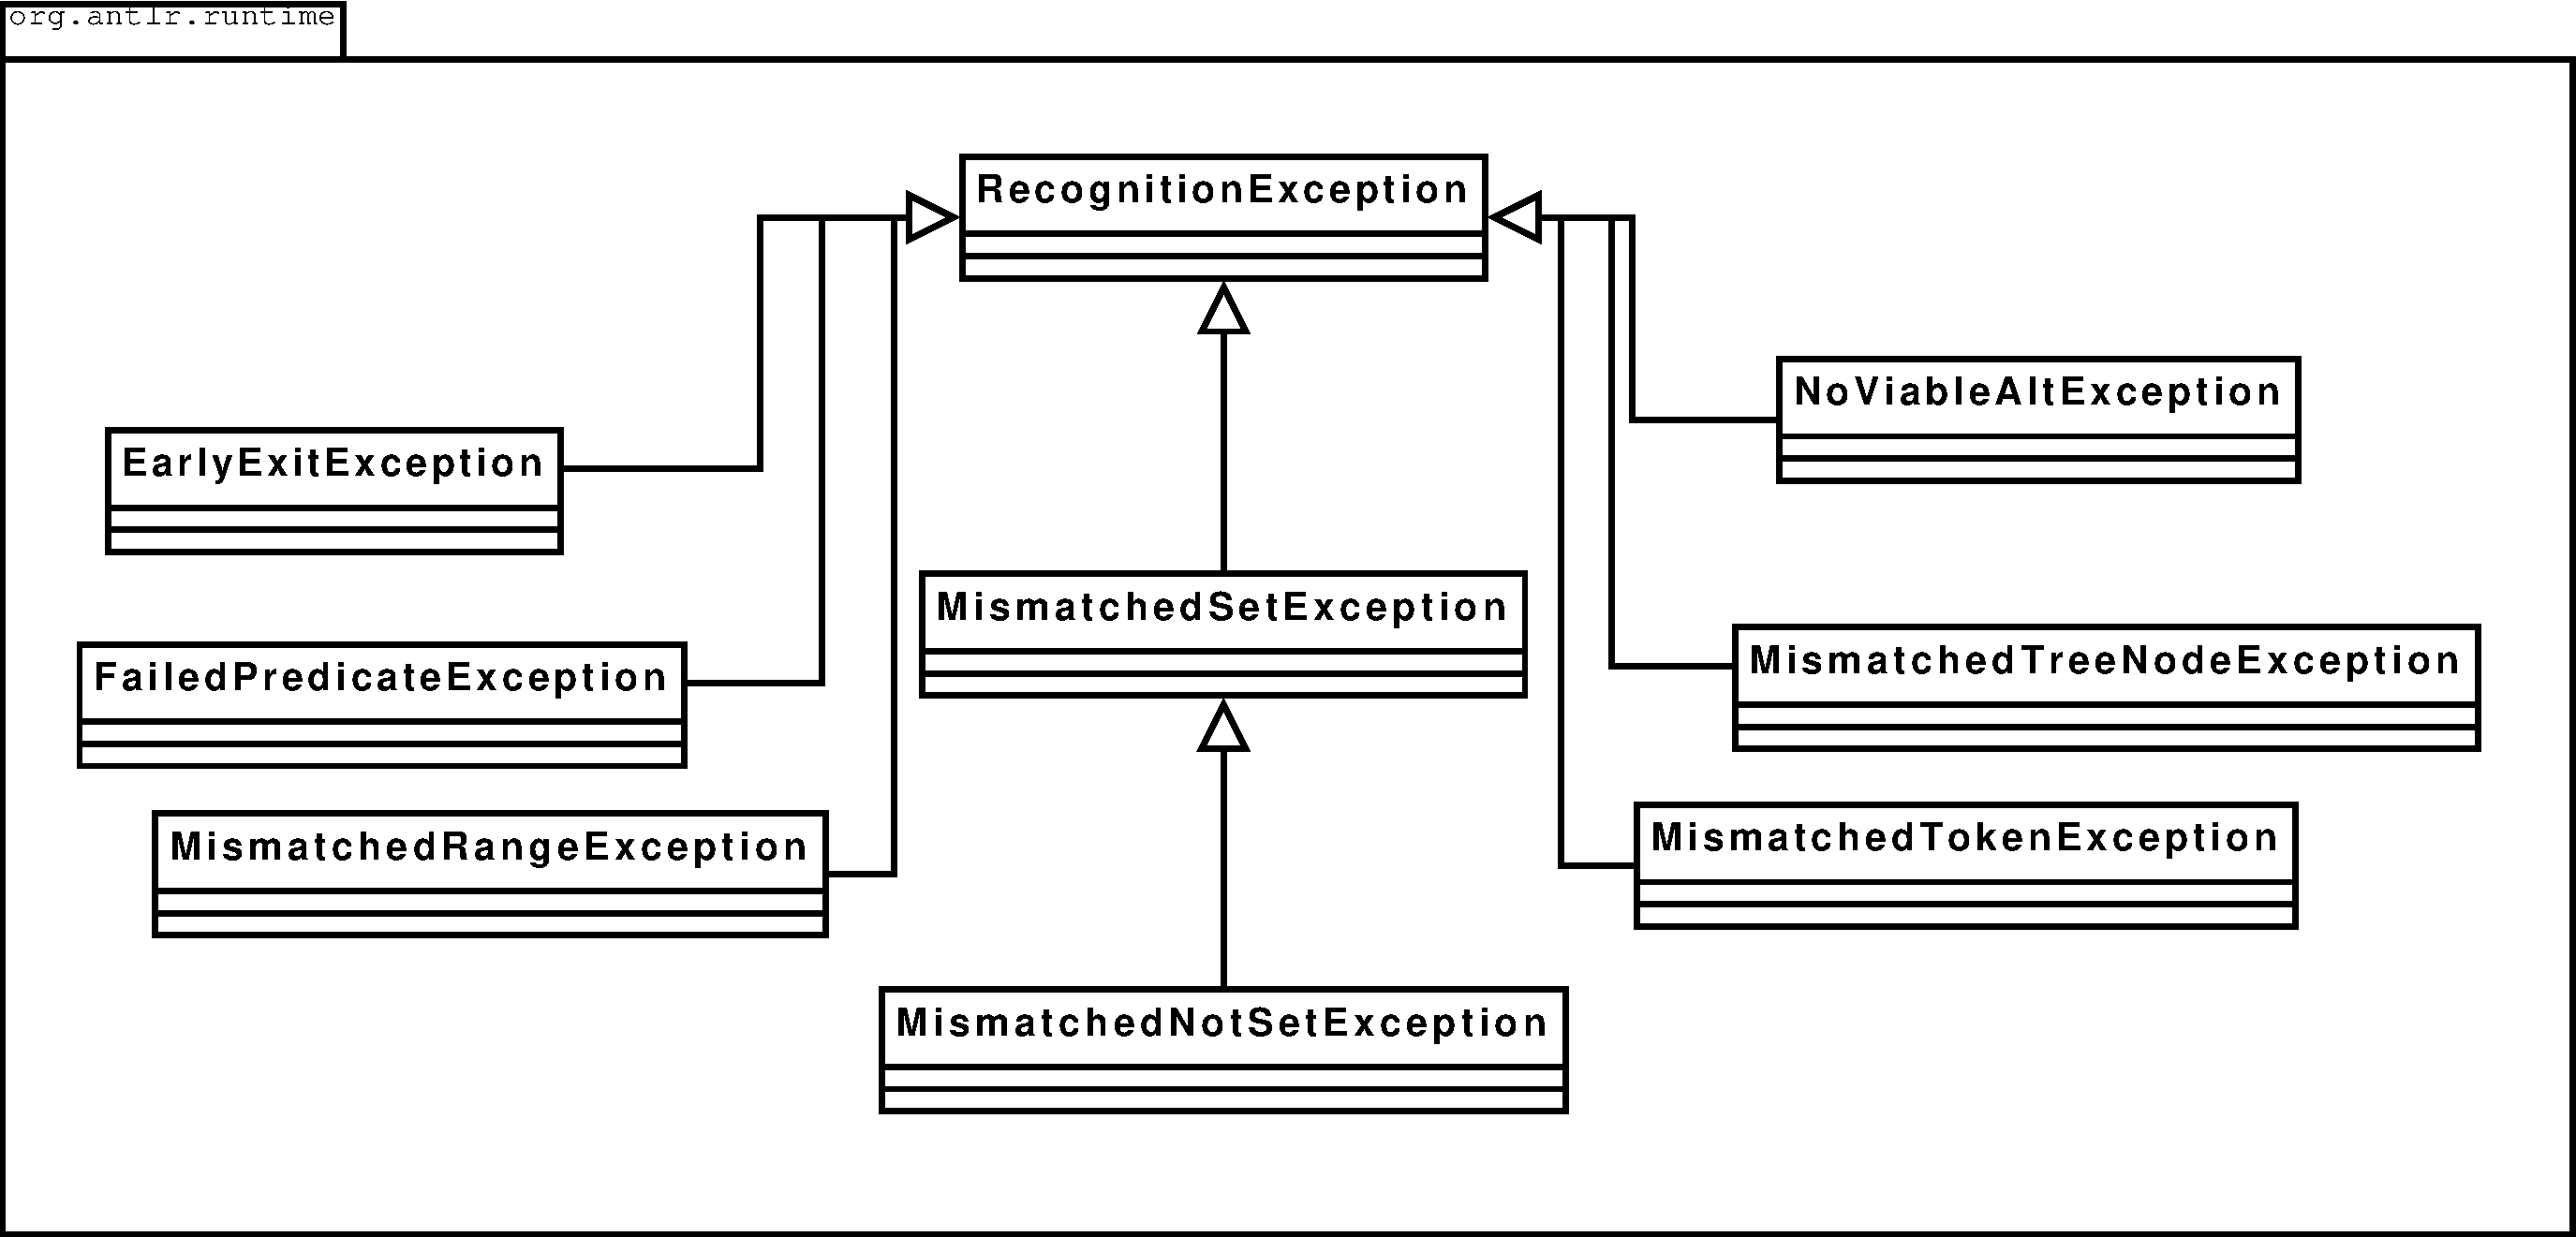
\includegraphics[width=1\textwidth]{diagrams/exception_uml}
  \caption{ANTLR exceptions class hierarchy}
\end{figure}
Error handling in ANTLR is initially done by catching exceptions and printing
an error message to stderr. The parser will then attempt to recover from the
error and continue parsing. This behaviour is not always desirable, so certain
methods were overridden to allow exceptions to be thrown upwards the stack to
the program that initiated the parser (the calling program, or top-level
program).

Specifically, this was done by overriding the methods \verb!mismatch()! as well as
\verb!recoverFromMismatchedSet()!, as such:

\begin{verbatim}
    protected void mismatch(IntStream input, 
                            int ttype, 
                            BitSet follow)
        throws RecognitionException
    {
        throw new MismatchedTokenException(ttype, input);
    }

    public void recoverFromMismatchedSet(IntStream input, 
                                         RecognitionException e, 
                                         BitSet follow)
        throws RecognitionException
    {
        throw e;
    }
\end{verbatim}

Additionally, a special \verb!@rulecatch! rule had to be added to force ANTLR from
handling errors and instead throwing the exceptions upwards:

\begin{verbatim}
@rulecatch {
    catch (RecognitionException e) {
        throw e;
    }
}
\end{verbatim}

However, some exceptions thrown by the lexer were impossible to handle - these
were handled by the \verb!nextToken()! method in the \verb!Lexer! superclass.
This issue has been documented in section 
\ref{sect:error_handling:syntax_errors}.
